%===============================================================================
% LaTeX sjabloon voor de bachelorproef toegepaste informatica aan HOGENT
% Meer info op https://github.com/HoGentTIN/latex-hogent-report
%===============================================================================


\documentclass[dutch,dit,thesis]{hogentreport}

% TODO:
% - If necessary, replace the option `dit`' with your own department!
%   Valid entries are dbo, dbt, dgz, dit, dlo, dog, dsa, soa
% - If you write your thesis in English (remark: only possible after getting
%   explicit approval!), remove the option "dutch," or replace with "english".

\usepackage{lipsum} % For blind text, can be removed after adding actual content
\usepackage{graphicx}

%% Pictures to include in the text can be put in the graphics/ folder
\graphicspath{{graphics/}}

%% For source code highlighting, requires pygments to be installed
%% Compile with the -shell-escape flag!
\usepackage[section]{minted}
\usemintedstyle{solarized-light}
\definecolor{bg}{RGB}{253,246,227} %% Set the background color of the codeframe

%% Change this line to edit the line numbering style:
\renewcommand{\theFancyVerbLine}{\ttfamily\scriptsize\arabic{FancyVerbLine}}

%% Macro definition to load external java source files with \javacode{filename}:
\newmintedfile[javacode]{java}{
    bgcolor=bg,
    fontfamily=tt,
    linenos=true,
    numberblanklines=true,
    numbersep=5pt,
    gobble=0,
    framesep=2mm,
    funcnamehighlighting=true,
    tabsize=4,
    obeytabs=false,
    breaklines=true,
    mathescape=false
    samepage=false,
    showspaces=false,
    showtabs =false,
    texcl=false,
}

% Other packages not already included can be imported here

%%---------- Document metadata -------------------------------------------------
% TODO: Replace this with your own information
\author{Dario Bronders}
\supervisor{Dhr. Manu De Buck}
\cosupervisor{Dhr. Geert van Boven}
\title[]%
    {Is AI geavanceerd genoeg om kunstwerken te genereren waarvan de boodschap herkenbaar is uit het dagelijks nieuws?}
\academicyear{\advance\year by -1 \the\year--\advance\year by 1 \the\year}
\examperiod{1}
\degreesought{\IfLanguageName{dutch}{Professionele bachelor in de toegepaste informatica}{Bachelor of applied computer science}}
\partialthesis{false} %% To display 'in partial fulfilment'
%\institution{Internshipcompany BVBA.}

%% Add global exceptions to the hyphenation here
\hyphenation{back-slash}

%% The bibliography (style and settings are  found in hogentthesis.cls)
\addbibresource{bachproef.bib}            %% Bibliography file
\addbibresource{../voorstel/voorstel.bib} %% Bibliography research proposal
\defbibheading{bibempty}{}

%% Prevent empty pages for right-handed chapter starts in twoside mode
\renewcommand{\cleardoublepage}{\clearpage}

\renewcommand{\arraystretch}{1.2}

%% Content starts here.
\begin{document}

%---------- Front matter -------------------------------------------------------

\frontmatter

\hypersetup{pageanchor=false} %% Disable page numbering references
%% Render a Dutch outer title page if the main language is English
\IfLanguageName{english}{%
    %% If necessary, information can be changed here
    \degreesought{Professionele Bachelor toegepaste informatica}%
    \begin{otherlanguage}{dutch}%
       \maketitle%
    \end{otherlanguage}%
}{}

%% Generates title page content
\maketitle
\hypersetup{pageanchor=true}

%%=============================================================================
%% Voorwoord
%%=============================================================================

\chapter*{\IfLanguageName{dutch}{Woord vooraf}{Preface}}%
\label{ch:voorwoord}

%% TODO:
%% Het voorwoord is het enige deel van de bachelorproef waar je vanuit je
%% eigen standpunt (``ik-vorm'') mag schrijven. Je kan hier bv. motiveren
%% waarom jij het onderwerp wil bespreken.
%% Vergeet ook niet te bedanken wie je geholpen/gesteund/... heeft
Deze bachelorproef markeert het hoogtepunt van mijn opleiding Bachelor in Toegepaste Informatica aan de Hogeschool Gent. Mijn fascinatie voor generatieve AI en automatisering, heeft geleid tot het idee om te onderzoeken of AI geavanceerd genoeg is om kunstwerken te genereren die een boodschap uit het dagelijks nieuws overbrengen. De mogelijkheden die deze technologieën bieden in het combineren van kunst, technologie en maatschappij hebben mij enorm gemotiveerd om dit onderzoek uit te voeren. \\
\\
Tijdens dit onderzoek heb ik kunnen rekenen op de waardevolle begeleiding en expertise van mijn promotor en co-promotor. Mijn oprechte dank gaat uit naar hen voor alle ondersteuning en tijd die zij in mij geïnvesteerd hebben om dit onderzoek tot een goed einde te brengen.
%%=============================================================================
%% Samenvatting
%%=============================================================================

% TODO: De "abstract" of samenvatting is een kernachtige (~ 1 blz. voor een
% thesis) synthese van het document.
%
% Een goede abstract biedt een kernachtig antwoord op volgende vragen:
%
% 1. Waarover gaat de bachelorproef?
% 2. Waarom heb je er over geschreven?
% 3. Hoe heb je het onderzoek uitgevoerd?
% 4. Wat waren de resultaten? Wat blijkt uit je onderzoek?
% 5. Wat betekenen je resultaten? Wat is de relevantie voor het werkveld?
%
% Daarom bestaat een abstract uit volgende componenten:
%
% - inleiding + kaderen thema
% - probleemstelling
% - (centrale) onderzoeksvraag
% - onderzoeksdoelstelling
% - methodologie
% - resultaten (beperk tot de belangrijkste, relevant voor de onderzoeksvraag)
% - conclusies, aanbevelingen, beperkingen
%
% LET OP! Een samenvatting is GEEN voorwoord!

%%---------- Nederlandse samenvatting -----------------------------------------
%
% TODO: Als je je bachelorproef in het Engels schrijft, moet je eerst een
% Nederlandse samenvatting invoegen. Haal daarvoor onderstaande code uit
% commentaar.
% Wie zijn bachelorproef in het Nederlands schrijft, kan dit negeren, de inhoud
% wordt niet in het document ingevoegd.

\IfLanguageName{english}{%
\selectlanguage{dutch}
\chapter*{Samenvatting}
\selectlanguage{english}
}{}

%%---------- Samenvatting -----------------------------------------------------
% De samenvatting in de hoofdtaal van het document

\chapter*{\IfLanguageName{dutch}{Samenvatting}{Abstract}}

Deze paper onderzoekt de mogelijkheid van het gebruik van AI om nieuwsverhalen om te zetten in visuele kunst. De focus ligt op de vraag in hoeverre AI effectief de essentie van een nieuwsverhaal kan vastleggen en vertalen naar visuele kunst. Daarnaast wordt onderzocht hoe technologieën zoals GPT (Generative Pre-trained Transformer) en DALL-E kunnen worden toegepast in de context van kunst, communicatie en maatschappij.\\

De onderzoeksvraag wordt beantwoord door middel van een combinatie van webscraping, waarbij nieuwsartikelen worden verzameld, en het gebruik van een GPT-model om de essentie van de nieuwsverhalen vast te leggen. Vervolgens wordt DALL-E ingezet om op basis van de gegenereerde prompts visuele kunstwerken te creëren.\\

De resultaten tonen aan dat AI in staat is om in zekere mate de essentie van een nieuwsverhaal om te zetten naar visuele kunst. Het juist formuleren van prompts en het voeren van een dialoog met het GPT-model zijn belangrijke aspecten voor het verkrijgen van gewenste resultaten. Echter, vanwege de abstracte aard van kunst en de subjectieve interpretatie ervan, is het niet altijd mogelijk om de boodschap van het nieuwsverhaal direct herkenbaar te maken in het gegenereerde kunstwerk.\\

Deze bevindingen hebben implicaties voor kunst, communicatie en maatschappij. AI-technologieën zoals GPT en DALL-E kunnen worden toegepast in de creatie van kunstwerken in kranten en nieuwswebsites. Daarnaast kunnen ze gebruikt worden voor het genereren van content in marketing, journalistiek en zakelijke communicatie. \\

Hoewel AI geavanceerd genoeg is om kunstwerken te genereren op basis van nieuwsverhalen, zijn er uitdagingen en beperkingen verbonden aan het proces. Het trainen van modellen met specifieke corpus van nieuwsartikelen kan helpen om betere resultaten te behalen. Webscraping is een effectieve methode om nieuwsartikelen te verzamelen, maar vereist regelmatige aanpassingen vanwege veranderingen in de structuur en lay-out van websites.\\

In conclusie biedt dit onderzoek inzicht in de mogelijkheden en beperkingen van AI bij het omzetten van nieuwsverhalen naar visuele kunst. Het benadrukt de waarde van de juiste formulering van prompts, de dialoog met het model en het begrip van de abstracte aard van kunst. Het biedt ook aanknopingspunten voor verdere onderzoeken naar optimalisatiestrategieën en toepassingen van AI in de kunst en communicatiesector.



%---------- Inhoud, lijst figuren, ... -----------------------------------------

\tableofcontents

% In a list of figures, the complete caption will be included. To prevent this,
% ALWAYS add a short description in the caption!
%
%  \caption[short description]{elaborate description}
%
% If you do, only the short description will be used in the list of figures

\listoffigures

% If you included tables and/or source code listings, uncomment the appropriate
% lines.
%\listoftables
%\listoflistings

% Als je een lijst van afkortingen of termen wil toevoegen, dan hoort die
% hier thuis. Gebruik bijvoorbeeld de ``glossaries'' package.
% https://www.overleaf.com/learn/latex/Glossaries

%---------- Kern ---------------------------------------------------------------

\mainmatter{}

% De eerste hoofdstukken van een bachelorproef zijn meestal een inleiding op
% het onderwerp, literatuurstudie en verantwoording methodologie.
% Aarzel niet om een meer beschrijvende titel aan deze hoofdstukken te geven of
% om bijvoorbeeld de inleiding en/of stand van zaken over meerdere hoofdstukken
% te verspreiden!

%%=============================================================================
%% Inleiding
%%=============================================================================

\chapter{\IfLanguageName{dutch}{Inleiding}{Introduction}}%
\label{ch:inleiding}

\noindent
In een wereld waarin technologie voortdurend evolueert, rijst de vraag of generatieve AI al geavanceerd genoeg is om betekenisvolle creaties te genereren die een boodschap overbrengen op basis van dagelijks nieuws. Deze bachelorproef onderzoekt de huidige stand van generatieve AI en beoordeelt de effectiviteit en kwaliteit van AI-generaties bij het communiceren van nieuwsgerelateerde boodschappen op unieke en boeiende wijze met het publiek. Door de combinatie van geavanceerde AI-technieken en automatisering van webscraping, verkennen we de grenzen van de interactie tussen technologie en informatievoorziening. Hierdoor bepalen we of generatieve AI al voldoende ontwikkeld is om deze uitdaging aan te gaan.
\pagebreak


\section{\IfLanguageName{dutch}{Context en achtergrond}{Context and background}}%
\label{sec:context}
\noindent
In de afgelopen jaren heeft AI aanzienlijke vooruitgang geboekt, met name op het gebied van generatieve modellen. Deze vooruitgang heeft geresulteerd in geavanceerde systemen die in staat zijn om zelfstandig creatieve output te genereren. Het potentieel van deze technologieën om kunst en communicatie te transformeren is enorm. Hieronder volgt een overzicht van de belangrijkste ontwikkelingen en trends op het gebied van generatieve AI. \\

\noindent
De relevantie van dit onderzoek ligt in de mogelijkheid om een brug te slaan tussen kunst, technologie en maatschappij. Het kan leiden tot nieuwe manieren van nieuwscommunicatie en artistieke expressie. De methodologie omvat het gebruik van AI en webscraping om kunstwerken te genereren op basis van actuele gebeurtenissen.


\section{\IfLanguageName{dutch}{Probleemstelling}{Problem Statement}}%
\label{sec:probleemstelling}
\noindent
Het is onduidelijk of AI geavanceerd genoeg is om kunstwerken te creëren die een nieuwsgerelateerde boodschap effectief overbrengen. Dit onderzoek zal deze vraag beantwoorden en de praktische toepassingen van dergelijke technologieën verkennen en gebruiken.

\section{\IfLanguageName{dutch}{Onderzoeksvraag}{Research question}}%
\label{sec:onderzoeksvraag}

\noindent
Kan AI geavanceerde kunstwerken genereren die een boodschap uit het dagelijks nieuws effectief overbrengen?

Deelvragen zijn onder andere:

\begin{itemize}
    \item Hoe kunnen technologieën zoals DALL-E en GPT-modellen worden toegepast in de context van kunst, communicatie en maatschappij?
    \item Hoe kan webscraping gebruikt worden om nieuwsartikelen te kunnen scrapen?
    \item In welke mate kan AI effectief de essentie van een nieuwsverhaal vastleggen en vertalen naar visuele kunst?
\end{itemize}

\pagebreak

\section{\IfLanguageName{dutch}{Onderzoeksdoelstelling}{Research objective}}%
\label{sec:onderzoeksdoelstelling}

\noindent
Het doel van deze bachelorproef is om de mogelijkheden van generatieve AI te onderzoeken bij het genereren van kunstwerken die nieuwsgerelateerde boodschappen overbrengen. Hierbij zal er specifiek worden onderzocht of generatieve AI al geavanceerd genoeg is om dergelijke kunstwerken te creëren en welke technieken hiervoor het meest geschikt zijn.  \\

Deze bachelorproef zal zich richten op kunstenaars, onderzoekers en bedrijven die geïnteresseerd zijn in de mogelijkheden van generatieve AI voor het creëren van betekenisvolle kunstwerken. Het doel van deze studie is om de haalbaarheid en effectiviteit van generatieve AI te onderzoeken bij het communiceren van nieuwsgerelateerde boodschappen door middel van kunst. 

\section{\IfLanguageName{dutch}{Opzet van deze bachelorproef}{Structure of this bachelor thesis}}%
\label{sec:opzet-bachelorproef}

% Het is gebruikelijk aan het einde van de inleiding een overzicht te
% geven van de opbouw van de rest van de tekst. Deze sectie bevat al een aanzet
% die je kan aanvullen/aanpassen in functie van je eigen tekst.

De rest van deze bachelorproef is als volgt opgebouwd: \\

In Hoofdstuk~\ref{ch:stand-van-zaken} wordt een overzicht gegeven van de stand van zaken binnen het onderzoeksdomein, op basis van een literatuurstudie. \\ 

Hoofdstuk~\ref{ch:methodologie} belicht de gebruikte methodologie en onderzoekstechnieken die zijn toegepast om de onderzoeksvragen te beantwoorden. \\ 

Hoofdstuk~\ref{ch:proof-of-concept} biedt een gedetailleerde uitleg over de implementatie van de applicatie, waarbij stap voor stap de ontwikkeling wordt besproken. \\ 

Hoofdstuk~\ref{ch:evaluatieproces} heeft als doel de geïnterpreteerde waarde van het schilderij te achterhalen door middel van een turingtest waarin we de resultaten bespreken.  \\

Tot slot wordt in Hoofdstuk~\ref{ch:conclusie} de conclusie gepresenteerd en worden de onderzoeksvragen beantwoord.
\chapter{\IfLanguageName{dutch}{Stand van zaken}{State of the art}}%
\label{ch:stand-van-zaken}

% Tip: Begin elk hoofdstuk met een paragraaf inleiding die beschrijft hoe
% dit hoofdstuk past binnen het geheel van de bachelorproef. Geef in het
% bijzonder aan wat de link is met het vorige en volgende hoofdstuk.

% Pas na deze inleidende paragraaf komt de eerste sectiehoofding.

Het genereren van kunstwerken op basis van tekstuele input heeft de afgelopen jaren aanzienlijke vooruitgang geboekt dankzij de opkomst van generatieve AI-technieken. Deze technieken maken gebruik van geavanceerde deep learning-algoritmen om kunstwerken te creëren die uniek zijn en vaak verrassend creatief. In deze literatuurstudie zullen we ons richten op de generatieve benadering van het creëren van kunstwerken, waarbij we dieper ingaan op de methoden en technieken die worden gebruikt om deze werken te genereren. \\

We zullen een uitgebreid overzicht geven van de huidige stand van zaken op het gebied van generatieve kunst, met specifieke nadruk op het gebruik van tekstuele input als basis voor het genereren van kunstwerken. We bespreken de evolutie van traditionele machinale vertaling en samenvatting naar de meer geavanceerde generatieve algoritmen die tegenwoordig worden toegepast. Door middel van deze algoritmen worden tekstinvoer omgezet in beelden, schilderijen, muziekstukken en andere vormen van kunst. \\

Binnen het domein van generatieve kunst zullen we specifiek kijken naar het gebruik van webscraping als een methode om tekstuele input te verzamelen voor het genereren van kunstwerken. We zullen de werking van deze methode bespreken, inclusief de uitdagingen die kunnen optreden bij het verkrijgen en verwerken van tekstuele gegevens van het web. Bovendien zullen we onderzoeken hoe webscraping kan worden toegepast om informatie te verzamelen die als input kan dienen voor het genereren van unieke en expressieve kunstwerken. \\

Al met al zal deze literatuurstudie een diepgaand inzicht bieden in de generatieve benadering van het creëren van kunstwerken op basis van tekstuele input. We zullen de huidige stand van de technologie onderzoeken, de potentie ervan in verschillende toepassingsgebieden bespreken en nadenken over mogelijke toekomstige ontwikkelingen op dit boeiende gebied.
\pagebreak


\section{Generatieve AI}

Generatieve AI is een subdomein van kunstmatige intelligentie dat zich richt op het creëren van nieuwe, unieke content op basis van bestaande gegevens. Het maakt gebruik van geavanceerde technieken zoals deep learning om patronen en relaties in de data te identificeren en te leren. Dit stelt de AI in staat om innovatieve en creatieve oplossingen te genereren voor verschillende toepassingen, zoals het genereren van kunstwerken op basis van tekstuele input \autocite{SonixAI2021}\\

Een voorbeeld van een toepassing van generatieve AI is het RobotReporter-project, uitgevoerd aan de Hogeschool Utrecht. Dit project onderzoekt de mogelijkheden van generatieve AI-systemen om journalistiek werk te automatiseren. Het project richt zich op het gebruik van webscraping en natural language processing (NLP) om informatie te verzamelen en te verwerken, en vervolgens met behulp van generatieve AI-algoritmen nieuwe content te creëren \autocite{HU2021}. Dit kan leiden tot efficiëntere en snellere nieuwsproductie. \\

Binnen de paper geschreven door Microsoft en OpenAI beschrijven ze de impact van generatieve AI op de arbeidsmarkt. Daarin wordt beschreven dat hoe langer en zwaardere studies je doet en dus hoe hoger het gemiddelde loon is binnen uw functie, hoe meer taken generatieve AI kan doen in plaats van de actor zelf. \autocite{gpt_micai} \\ 

Generatieve AI heeft niet alleen invloed op de hogerbetaalde jobs, maar ook op andere beroepen. Een artikel van Harvard Business Review bespreekt de impact van generatieve AI op klantenserviceberoepen \autocite{HBR2023}. In plaats van banen te vervangen, wordt betoogd dat generatieve AI klantenservicemedewerkers kan ondersteunen en hun werk kan verbeteren. Door geautomatiseerde systemen te gebruiken om routineuze taken te voltooien, kunnen medewerkers zich concentreren op meer complexe en empathische aspecten van hun werk. \\

In de afgelopen jaren is generatieve AI een veelbelovend onderzoeksgebied geworden, met tal van toepassingen en mogelijkheden. Desondanks zijn er nog steeds uitdagingen en beperkingen die moeten worden aangepakt, zoals de  aspecten en de benodigde rekenkracht. Toekomstig onderzoek en ontwikkeling zullen waarschijnlijk leiden tot nieuwe doorbraken en toepassingen op het gebied van generatieve AI. \\

\subsection{Transformer}
Stel je voor dat je een groep vrienden hebt die allemaal tegelijkertijd praten. Je kunt aandacht besteden aan iedereen, maar afhankelijk van het onderwerp, zul je misschien meer aandacht besteden aan wat sommigen zeggen dan aan anderen. Dit is hoe transformers werken. \\

Transformers zijn een soort computermodel dat wordt gebruikt om taal te begrijpen en te genereren. In plaats van elk woord in een zin een voor een te verwerken, zoals een mens die leest, kunnen transformers naar alle woorden in een zin tegelijk kijken. Dit stelt hen in staat om de relaties tussen woorden beter te begrijpen, ongeacht hoe ver ze in de zin van elkaar verwijderd zijn. \\

Laten we een voorbeeld nemen: "Het glas brak omdat het gevallen was." Voor ons is het duidelijk dat "het" verwijst naar "het glas". Maar voor een computermodel dat woorden een voor een verwerkt, kan het moeilijk zijn om deze verbinding te maken, vooral als de zin langer is. Transformers lossen dit probleem op met iets dat we "attention" noemen. Dit betekent dat het model beslist welke delen van de zin het belangrijkst zijn om de betekenis te begrijpen, net zoals jij zou besluiten naar wie je moet luisteren in een groep vrienden.\\ 

Dit mechanisme van "attention" is niet alleen cruciaal voor het begrijpen van tekst, maar ook voor het genereren ervan, zoals in het geval van GPT. \\

GPT,, is in feite een groot transformer-model dat is getraind op een aanzienlijke hoeveelheid tekst van het internet. Tijdens deze training heeft het model een verscheidenheid aan gesprekken en schrijfstijlen 'gehoord', en met behulp van de transformer-architectuur, heeft het de onderlinge relaties tussen woorden in deze teksten leren begrijpen. \\

\subsection{GPT}
Generative Pre-trained Transformer (GPT) is een reeks taalmodellen ontwikkeld door OpenAI. Deze modellen zijn ontworpen om menselijke taal te begrijpen en te genereren met een hoge mate van nauwkeurigheid en coherentie. De reeks GPT-modellen omvat GPT-3, GPT-3.5 en GPT-4. GPT-modellen zijn relevant voor de vraag of AI in staat is kunstwerken te genereren die niet van echt te onderscheiden zijn, vanwege hun prestaties op het gebied van natuurlijke taalverwerking en tekstgeneratie. \\

In de volgende subsecties zullen we de kenmerken en prestaties van elk model bespreken, evenals hun bijdragen aan het veld van kunstmatige intelligentie en hun potentieel om kunstwerken te helpen genereren. \\

\subsubsection{GPT-3}
GPT-3, is een transformer-gebaseerd taalmodel met 175 miljard parameters. Het model heeft interessante prestaties geleverd op het gebied van natuurlijke taalverwerking en kan tekst genereren. \autocite{nytimes_gpt3}. GPT-3 kan worden gebruikt om teksten te genereren, zoals nieuwsartikelen, verhalen, gedichten en zelfs code. Hoewel het model niet perfect is en soms onjuiste of irrelevante informatie kan genereren, heeft het de aandacht getrokken van onderzoekers, technologiebedrijven en het grote publiek vanwege de veelzijdigheid en de kwaliteit van de gegenereerde tekst \autocite{wiki_gpt3}. \\

GPT-3 is gelanceerd door OpenAI en heeft een ongekende groei doorgemaakt, met een recordaantal gebruikers in korte tijd. Binnen slechts twee maanden na lancering bereikte het platform 100 miljoen gebruikers, waarmee het één van de snelst groeiende platform ooit is \ref{fig:gpt_growth}. \autocite{reuters_chatgpt}. Deze snelle groei en brede acceptatie zijn indicatief voor de potentie en relevantie van GPT-3 voor deze paper.\\

\begin{center}
    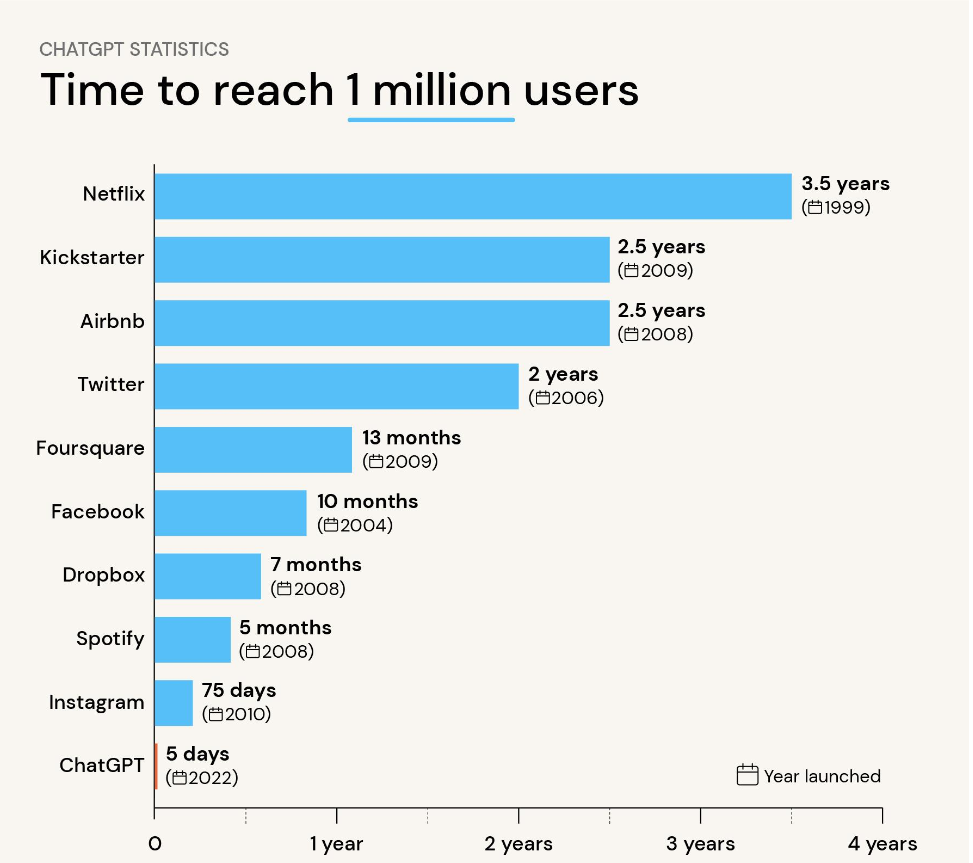
\includegraphics[width = 4in]{gpt_growth.png}
    \captionof{figure}{Tijd nodig tot 1 milioen gebruikers. \autocite{gpt_millie}}
    \label{fig:gpt_growth}
\end{center}

GPT-3 heeft een API die gebruikt kan worden.

\subsubsection{GPT-3.5}
GPT-3.5, een geüpgradede versie van het GPT-3-model, biedt geavanceerdere taalbegrip- en generatiecapaciteiten in vergelijking met zijn voorganger. De verbeteringen in GPT-3.5 stellen het model in staat om een breder scala aan complexe taken uit te voeren en betere resultaten te leveren in verschillende toepassingsgebieden, zoals tekstclassificatie, sentimentanalyse, tekstgeneratie en contextueel begrip \autocite{gpt_nappier, gpt_cn}. \\

\autocite{gpt_nappier} bespreken de technische aspecten van GPT-3.5 en de belangrijkste verschillen tussen GPT-3 en GPT-3.5. Een van de opmerkelijke verbeteringen in GPT-3.5 is het vermogen om context beter te begrijpen en relevante tekst te genereren op basis van die context. Dit is vooral belangrijk in taken waarbij contextuele informatie cruciaal is voor het begrijpen en genereren van geschikte antwoorden of voortzettingen van een tekst. \\

Een ander belangrijk aspect van GPT-3.5 is de verbeterde efficiëntie en prestaties. GPT-3.5 maakt gebruik van geoptimaliseerde architecturen en trainingsmethoden om de modelgrootte en computatievereisten te verminderen zonder concessies te doen aan de prestaties. Dit maakt het model toegankelijker en bruikbaarder voor een breder scala aan toepassingen en apparaten \autocite{gpt_nappier}. \\

\autocite{gpt_cn} verkennen de toepassingsmogelijkheden van GPT-3.5 en presenteren verschillende casestudy's die de prestaties en effectiviteit van het model aantonen. Ze onderzoeken het gebruik van GPT-3.5 in diverse domeinen, zoals het genereren van nieuwsartikelen, samenvatten van teksten, het beantwoorden van vragen op basis van tekst en het genereren van code. \\

Ondanks de goede prestaties van GPT-3.5, zijn er nog steeds uitdagingen en beperkingen die moeten worden aangepakt. In \autocite{gpt_cn} worden enkele van deze problemen besproken, zoals het genereren van irrelevante of onjuiste informatie (hallucineren), gevoeligheid voor vooroordelen in de trainingsdata en het vermogen om lange teksten te genereren zonder af te dwalen van het onderwerp. Toekomstig onderzoek zou zich kunnen richten op het verbeteren van deze aspecten en het ontwikkelen van methoden om de modelprestaties verder te verfijnen.\\

GPT-3.5 heeft een API die gebruikt kan worden onder de naam gpt-3.5-turbo. 

\subsubsection{GPT4}
GPT-4, de opvolger van GPT-3.5, is een nog geavanceerder transformer-gebaseerd taalmodel dat verder bouwt op de successen en verbeteringen van zijn voorgangers. GPT-4 biedt aanzienlijke verbeteringen op het gebied van natuurlijke taalverwerking, tekstgeneratie en begrip, evenals efficiëntie en bruikbaarheid \autocite{gpt_openai, gpt_micai}. \\

Een belangrijk kenmerk van GPT-4 is het vermogen om nog nauwkeuriger en coherenter menselijke taal te genereren en te begrijpen. Hierdoor kan GPT-4 beter presteren in verschillende toepassingsgebieden, zoals tekstclassificatie, sentimentanalyse, tekstgeneratie, contextueel begrip en vele anderen \autocite{gpt_micai}. \\

\autocite{gpt_cn} onderzoeken de technische aspecten en verbeteringen van GPT-4 ten opzichte van GPT-3.5. Ze benadrukken de geoptimaliseerde architecturen en trainingsmethoden die in GPT-4 zijn geïmplementeerd, waardoor het model betere prestaties kan leveren zonder dat dit ten koste gaat van de efficiëntie. Deze verbeteringen maken GPT-4 toegankelijker en bruikbaarder voor een breder scala aan toepassingen en apparaten. \\

Binnen het onderzoek van Microsoft \autocite{gpt_micai} toont men aan dat GPT-4 vormen van algemene intelligentie vertoont. Dit blijkt uit de kerncapaciteiten, zoals redeneren, creativiteit en deductie, expertise op verschillende onderwerpen, en de verscheidenheid aan taken die het kan uitvoeren. Hoewel er nog veel werk te doen is om een volledige AGI (Artificial General Intelligence) te creëren, wordt benadrukt dat het definiëren van intelligentie, AI en AGI complex en controversieel is en dat er geen definitieve definitie bestaat. Het onderzoek suggereert dat toekomstig werk op het gebied van GPT-4 en vergelijkbare systemen zich kan richten op het verkennen van nieuwe toepassingen en domeinen en het begrijpen van de mechanismen en principes die aan hun intelligentie ten grondslag liggen. \\

Naast de prestaties van GPT-4 hebben Elon Musk en andere experts opgeroepen tot een tijdelijke stop van Large Language Models (LLM) zoals GPT-4 kunnen overtreffen, vanwege potentiële risico's en onvoorziene gevolgen die dergelijke geavanceerde systemen met zich mee kunnen brengen zonder \autocite{reuters_musk}. 
 
\section{AI-gegenereerde kunst: tools en voorbeelden}
\subsection{ Midjourney}
Midjourney is een organisatie die met behulp van discord kunstwerken kan genereren, zo kun je een prompt sturen in de chat en krijg je verschillende kunstwerken te zien op basis van je prompt, indien je tevreden bent met de resultaten kun je de foto in hoge resultatie downloaden. Indien niet, kun je de beste van de X-aantal resultaten selecteren en hierop nieuwe resultaten laten genereren. 

\begin{center}
    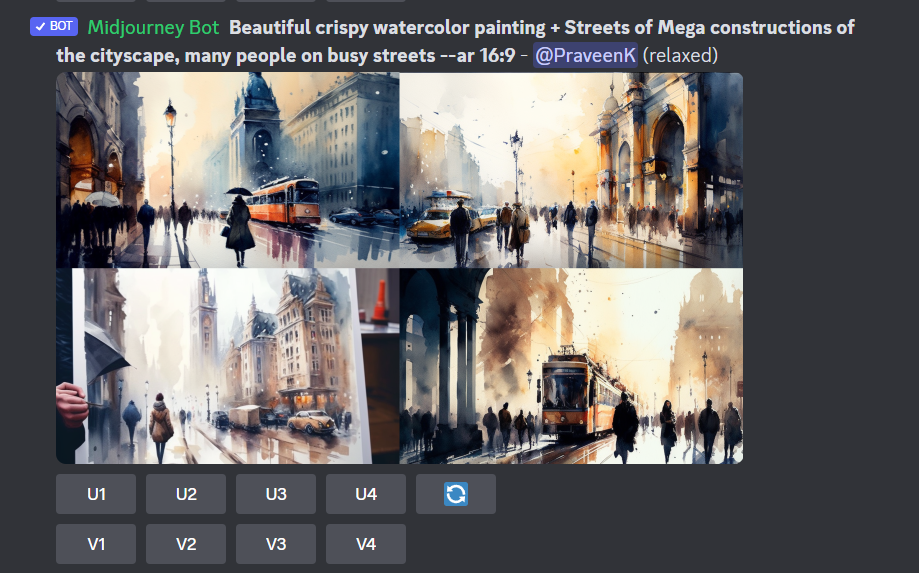
\includegraphics[width = 4in]{midjourney_ex.png}
    \captionof{figure}{Voorbeelden van AI-gegenereerde kunstwerken met behulp van Midjourney.}
    \label{fig:midjourney_ex.png}
\end{center}

Midjourney heeft geen API die we kunnen gebruiken.

\subsection{ Dall-E}
Dall-E kan gebruikt worden op de website om kunstwerkente generen maar met extra functionaliteiten vergeleken met midjourney. Dall-E laat het toe om foto's te editen en varianties van een kunstwerk te vragen. Met editen kun je een plaats markeren op het gegenereerde resultaat en hierop een nieuwe promp laten genereren, op deze manier kun je bepaalde dingen aanpassen of nieuwe attributen laten genereren op het kunstwerk. \\

Hieronder vindt u het resultaat gegenereerd op de prompt: ``Painted by Dali: Taiwan targeted by China'.' \\

\begin{figure}[h!]
    \centering
    \begin{tabular}{llll}
        
\includegraphics[width = 1.5in]{dall-e_ex1.png} &
        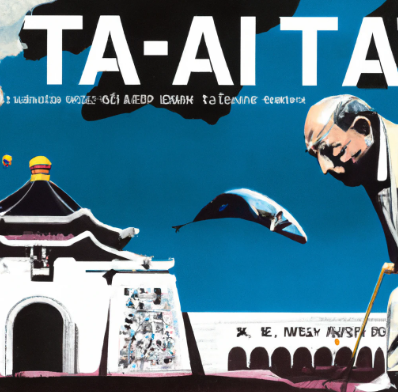
\includegraphics[width = 1.5in]{dall-e_ex2.png} \\
        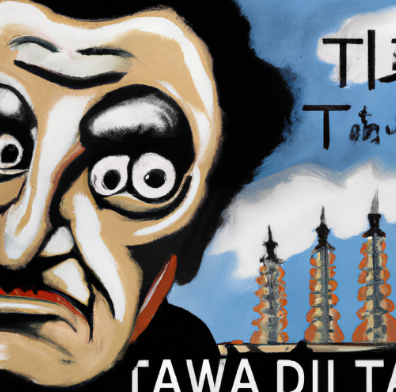
\includegraphics[width = 1.5in]{dall-e_ex3.png} &
        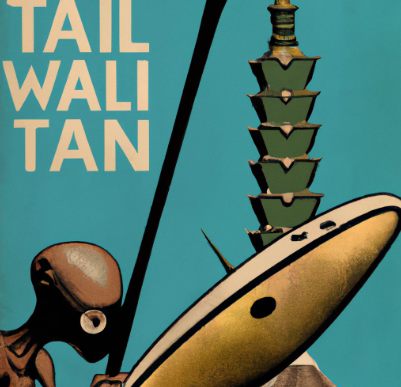
\includegraphics[width = 1.5in]{dall-e_ex4.png}
    \end{tabular}
    \caption{Voorbeelden van AI-gegenereerde kunstwerken met behulp van Dall-E.}
    \label{fig:examples}
\end{figure}


 Bovenstaande functionaliteiten worden ook aangeboden binnen de API van OpenAI.
\pagebreak

\subsection{Stable Diffusion}
Met Stable Diffusion kun je 1-4 kunstwerken laten genereren. \\

Hieronder vind u het resultaat gegenereerd op de prompt:  ``Painted by Van Gogh: War in Russia, food crisis in Asia.''

\begin{figure}[h!]
    \centering
    \begin{tabular}{llll}
        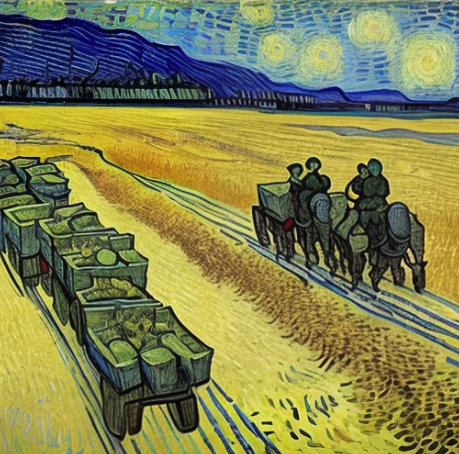
\includegraphics[width = 1.5in]{sd_ex1.png} &
        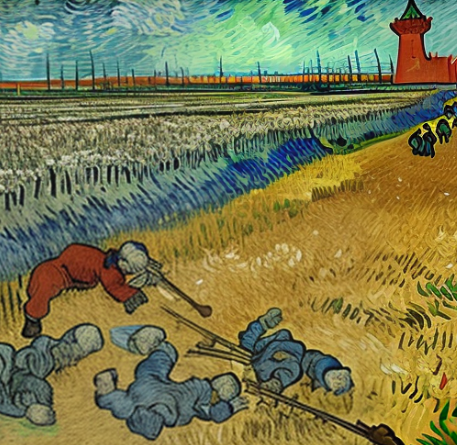
\includegraphics[width = 1.5in]{sd_ex2.png} \\
        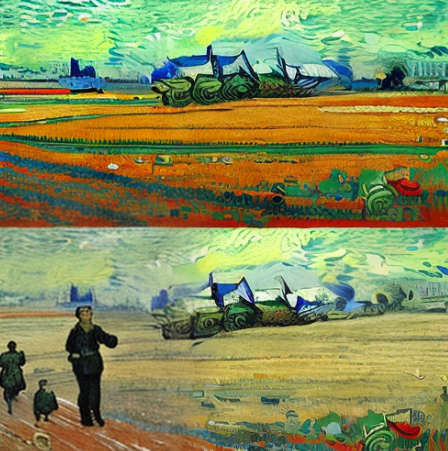
\includegraphics[width = 1.5in]{sd_ex3.png} &
        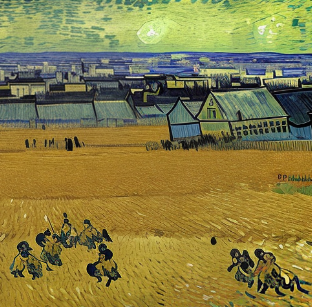
\includegraphics[width = 1.5in]{sd_ex4.png}
    \end{tabular}
    \caption{Voorbeelden van AI-gegenereerde kunstwerken met behulp van Stable Diffusion.}
    \label{fig:examples}
\end{figure}

Stable Diffusion heeft een API waarvan gebruik van gemaakt kan worden. \\

\pagebreak

\subsection{Toepassingen}
Binnen deze subsectie bespreek ik enkele toepassingen die gebruik maken van de eerder vermelde tools in punt 2.1/2.2 en 2.3.

\subsubsection{NFT's}
Een non-fungible token, beter bekend als een NFT, is een uniek digitaal object op een blockchain, meestal verbonden met speciale digitale content zoals foto's of muziek. Ze hebben een gigantische markt opgebouwd, waar individuele NFT's een waarde van miljoenen dollars kunnen bereiken \autocite{nft_whatisit}. \\

LLM's hebben het potentieel om de markt te verstoren op een manier die het menselijke aspect van NFT's kan wegnemen. In plaats van kunstenaars en creatievelingen die unieke digitale content maken, kunnen we een toekomst zien waarin AI de 'creator' wordt, wat de menselijke inspanning, creativiteit en originaliteit die traditioneel geassocieerd worden met kunst kan ondermijnen. 

\subsubsection{Graphic Design}
Binnen het domein van graphic design kunnen AI-tools zoals DALL-E en StyleGAN worden ingezet voor verschillende toepassingen. Zo kunnen ze bijvoorbeeld worden gebruikt om nieuwe verpakkingen, zoals cornflakesdozen, te ontwerpen door unieke en aantrekkelijke ontwerpen te genereren op basis van bestaande stijlen en trends.  \\

Daarnaast kunnen ze bedrijven helpen bij het creëren van opvallende en herkenbare logo's door verschillende concepten te genereren op basis van tekstbeschrijvingen of bestaande ontwerpelementen. 

\subsubsection{Webdevelopers}
Voor frontend webdevelopers kunnen AI-tools zoals Midjourney bijzonder handig zijn bij het opdoen van inspiratie voor het ontwerpen van websites. Door bijvoorbeeld aan Midjourney een prompt te geven zoals "Beautiful landing page Blissful state of mind, Natural healing techniques, Yoga, Meditation, ui, ux, elementor, wordpress, simple, minimalistic, aesthetics" \ref{fig:frontendwebdev_ex}, kan de AI-tool een reeks ontwerpen en concepten genereren die passen bij de gegeven beschrijving. Dit helpt webdevelopers om ideeën op te doen en hun creativiteit te stimuleren bij het bouwen van unieke en aantrekkelijke websites.

\begin{center}
    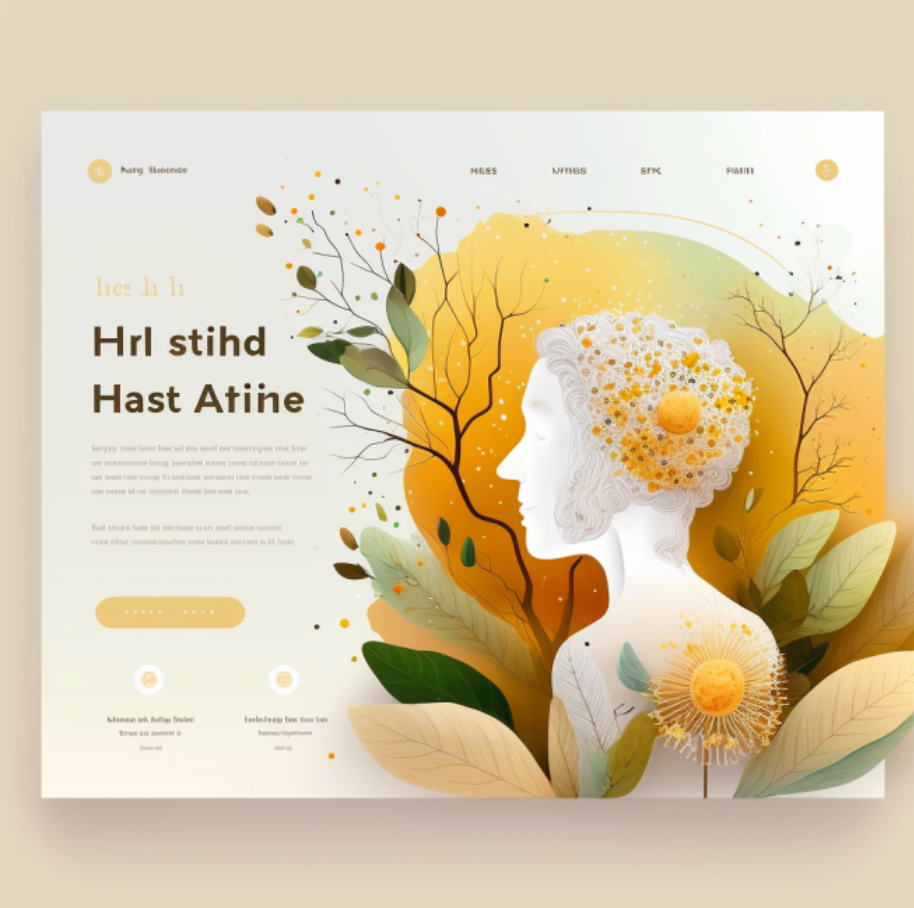
\includegraphics[width = 4in]{frontendwebdev_ex}
    \captionof{figure}{Voorbeeld: Landingspagina op basis van een prompt in Midjourney.}
    \label{fig:frontendwebdev_ex}
\end{center}


\section{Webscraping}
Webscraping is een krachtige techniek die gebruikt kan worden om tekstuele input te verzamelen voor het genereren van kunstwerken. Met webscraping kunnen gegevens van websites worden geëxtraheerd en gebruikt worden als input voor generatieve AI-algoritmen om kunstwerken te genereren. \\
 
Een belangrijke overweging bij het gebruik van webscraping voor het genereren van kunstwerken is het respecteren van de regels en beperkingen van de websites die worden gescraped. Websites kunnen bijvoorbeeld beperkingen opleggen via het robots.txt-bestand, dat aangeeft welke delen van de website geopend kunnen worden voor scraping. Het is belangrijk om deze regels te respecteren en alleen gegevens te verzamelen waarvoor toestemming is verleend. \\

Belangrijke zaken waarmee er rekening gehouden moet worden om een scraper te creeëren volgens \autocite{BIO2014}:

\begin{itemize}
    \item \textbf{Toegang krijgen tot de site:} De webscraper maakt verbinding met de doelwebsite via het HTTP-protocol en houdt rekening met verzoeksmethoden zoals GET en POST. Daarnaast moet de 'User-Agent' correct worden ingesteld.
    \item \textbf{HTML-Parsen en de inhoud extraheren:} De scraper moet in staat zijn om de HTML-structuur van de webpagina te begrijpen en de relevante gegevens te extraheren. Dit kan worden bereikt met behulp van reguliere expressies, HTML-parsing bibliotheken of op selectors gebaseerde talen zoals XPath en CSS-selector syntax.
    \item \textbf{Output:} De geëxtraheerde gegevens moeten worden omgezet in een gestructureerde weergave die geschikt is voor verdere analyse en opslag, zoals in-memory datastructuren of tekstgebaseerde bestandsformaten zoals XML of CSV.
\end{itemize}

\subsection{Ethische aspecten}
\label{subsection:scraper-ethische-aspecten}
Bij het uitvoeren van webscraping-activiteiten is het van belang om ethische overwegingen in acht te nemen. Webscraping kan verschillende ethische uitdagingen met zich meebrengen, zoals het respecteren van de privacy van gebruikers en het naleven van de regels en beperkingen van websites. Hier zijn enkele belangrijke ethische aspecten volgens \autocite{scrape_ethics} om rekening mee te houden tijdens het ontwikkelen van de scraper: 

\begin{itemize}
    \item \textbf{Privacy en persoonlijke gegevens:} Het is essentieel om geen persoonlijke identificeerbare informatie of gevoelige gegevens te verzamelen zonder de toestemming van de gebruikers of de website-eigenaren.
    \item \textbf{Auteursrecht en intellectuele eigendom:} Het is belangrijk om de regels en beperkingen van websites te respecteren met betrekking tot het gebruik en de reproductie van hun inhoud.
    \item \textbf{Serverbelasting:} Webscraping kan de serverbelasting van websites verhogen, vooral als grote hoeveelheden gegevens worden opgevraagd of als frequent en intensief scraping plaatsvindt. Dit kunnen we vermijden door een wachttijd te simuleren na elke request. 
\end{itemize}

\subsection{BeautifulSoup4}
BeautifulSoup4 (BS4) is een populaire Python-bibliotheek voor webscraping die het eenvoudig maakt om gegevens van webpagina's te verkrijgen en te verwerken \autocite{BIO2014, BSFOR2015}. \\

Het biedt een intuïtieve en eenvoudige manier om HTML- en XML-documenten te parseren en gegevens eruit te extraheren. Met BeautifulSoup4 kunnen ontwikkelaars elementen selecteren op basis van tags, klassen, ids en andere attributen. Ze kunnen ook door de hiërarchie van de HTML-structuur navigeren en de gewenste gegevens extraheren. \\

De officiële documentatie van BeautifulSoup4 is een waardevolle bron van informatie en richtlijnen voor het gebruik van de bibliotheek. Het bevat gedetailleerde uitleg, voorbeelden en referenties naar de verschillende functies en methoden van BeautifulSoup4. 
De documentatie is beschikbaar op de volgende website: \autocite{BS4Documentation}. \\


\section{De uitdagingen en beperkingen van AI-gegenereerde kunst}
AI-gegenereerde kunst brengt verschillende uitdagingen en beperkingen met zich mee, die invloed hebben op de creativiteit, originaliteit en interpretatie van de gegenereerde kunstwerken en dus ook het onderzoek zelf.

\subsection{Creativiteit}
Een van de belangrijkste uitdagingen bij AI-gegenereerde kunst is het stimuleren van creativiteit. Hoewel AI in staat is om grote hoeveelheden gegevens te analyseren en patronen te herkennen, mist het vaak de menselijke verbeeldingskracht en intuïtie die nodig zijn voor het creëren van originele en innovatieve kunstwerken. AI-algoritmen zijn gebaseerd op bestaande gegevens en modellen, waardoor ze vaak geneigd zijn om bestaande stijlen en trends te repliceren in plaats van iets volledig nieuws te creëren. Het uitdagen van AI om buiten de gebaande paden te denken en echt unieke kunstwerken te genereren, blijft een grote uitdaging.

\subsection{Originaliteit}
Een andere beperking van AI-gegenereerde kunst is de kwestie van originaliteit. Omdat AI-systemen zijn getraind op bestaande datasets, bestaat het risico dat ze onbedoeld bestaande kunstwerken of ideeën reproduceren zonder voldoende originaliteit toe te voegen. Dit kan leiden tot het genereren van kunstwerken die sterk lijken op bestaande werken of het schenden van auteursrechten. Het waarborgen van voldoende originaliteit in AI-gegenereerde kunst vereist een zorgvuldige afweging tussen het gebruik van bestaande gegevens voor training en het aanmoedigen van nieuwe, unieke expressie.

\subsection{Interpretatie}
Een uitdaging bij het omgaan met AI-gegenereerde kunst is de interpretatie ervan. Omdat kunstwerken vaak worden geassocieerd met emotie, betekenis en subjectiviteit, kan de interpretatie van AI-gegenereerde kunstwerken een uitdaging zijn. Het ontbreekt AI vaak aan de menselijke context en begrip om diepere betekenissen en nuances in kunstwerken te begrijpen. Dit kan resulteren in kunstwerken die voor mensen moeilijk te interpreteren zijn of die niet de gewenste emotionele impact hebben. Het betrekken van menselijke interactie en interpretatie bij AI-gegenereerde kunst kan helpen om deze uitdaging aan te pakken en een meer gelaagde en betekenisvolle ervaring te creëren.

Het is belangrijk om deze uitdagingen en beperkingen in gedachten te houden bij het ontwikkelen en evalueren van AI-gegenereerde kunst. Door voortdurend te streven naar creativiteit, originaliteit en begrijpelijke interpretatie, kunnen we de potentie van AI benutten om nieuwe vormen van artistieke expressie te verkennen en te ontwikkelen.

%%=============================================================================
%% Methodologie
%%=============================================================================

\chapter{\IfLanguageName{dutch}{Methodologie}{Methodology}}%
\label{ch:methodologie}

%% TODO: Hoe ben je te werk gegaan? Verdeel je onderzoek in grote fasen, en
%% licht in elke fase toe welke stappen je gevolgd hebt. Verantwoord waarom je
%% op deze manier te werk gegaan bent. Je moet kunnen aantonen dat je de best
%% mogelijke manier toegepast hebt om een antwoord te vinden op de
%% onderzoeksvraag.
\section{Inleiding}
Het onderzoek begint met een grondige literatuurstudie die te vinden is in Hoofdstuk 2. Deze literatuurstudie bepaalt de onderwerpen waarop dit onderzoek zich zal richten en onderzoekt enkele belangrijke en veelvoorkomende webscraping- en AI-modellen die momenteel beschikbaar zijn.  \\

\section{Fases}
\begin{itemize}
    \item \textbf{Fase 1}: Ontwikkelen van een webscraper die in staat is om de website, titel op een correct en gestructureerde manier te verzamelen. 
    \item \textbf{Fase 2}: Prompt genereren met GPT met behulp van de verzamelde artikels. 
    \item \textbf{Fase 3}: Genereren van een kunstwerk met DALL-E op basis van de prompt uit vorige fase 2.
\end{itemize} 

\section{Onderverdeling}

Hoofdstuk \ref{ch:proof-of-concept}  beschrijft de proof-of-concept van het onderzoek. Het bevat de ontwikkeling van de webscraper in fase 1 en het gebruik van de verzamelde artikelen als input voor het GPT en DALL-E model in fase 2 en 3. Er zal uitgelegd worden hoe de gegenereerde prompts dienen als basis voor het genereren van schilderijen met behulp van DALL-E. Het doel van dit hoofdstuk is om de implementatie en werking van de applicatie aan te tonen op basis van de verkregen informatie uit hoofdstuk \ref{ch:stand-van-zaken}.  \\

Hoofdstuk beschrijft \ref{ch:evaluatieproces} de evaluatieproces van het gegenereerde kunstwerk. In dit hoofdstuk wordt er een evaluatieproces beschreven dat de te geïnterpreteerde waarde van het schilderij achterhaalt. Dit zal gedaan worden aan de hand van een turingtest waar we de deelnemers zullen bevragen om een boodschap uit een schilderij te halen. (of een nieuwsartikel hieraan te koppelen) Met behulp van deze turingtest kunnen we bepalen of AI in staat is om de boodschap van het nieuws over te brengen.




% Voeg hier je eigen hoofdstukken toe die de ``corpus'' van je bachelorproef
% vormen. De structuur en titels hangen af van je eigen onderzoek. Je kan bv.
% elke fase in je onderzoek in een apart hoofdstuk bespreken.

%\input{...}
%\input{...}
%...

%%=============================================================================
%% Conclusie
%%=============================================================================

\chapter{Conclusie}%
\label{ch:conclusie}
In dit onderzoek werd een antwoord gegeven op de hoofdonderzoeksvraag en deelvragen. En lichten we kort toe over mogelijke toekomstige onderzoeksmogelijkheden. 

We beginnen met een antwoord te bieden op de deelvragen omdat deze een betere context en inzicht zullen geven voor de onderzoeksvraag. 

\section{\IfLanguageName{dutch}{Deelvraag: In welke mate kan AI effectief de essentie van een nieuwsverhaal vastleggen en vertalen naar visuele kunst?}{Sub-question: To what extent can AI effectively capture the essence of a news story and translate it into visual art?}}%

In mijn mening en wat blijkt uit de turingtest kan AI in zekere mate effectief de essentie van een nieuwsverhaal vastleggen en vertalen naar visuele kunst. Het belangrijkste aspect is het gebruik van de juiste prompts bij GPT om de gewenste resultaten te verkrijgen. Het komt echter voor dat tijdens de conversatie GPT niet altijd in staat is om het hoogtepunt van het nieuwsverhaal weer te geven waar de kenmerken duidelijk zichtbaar zijn. Daarom is het van cruciaal belang om goede prompts te gebruiken en de conversatie met het model aan te gaan. \\

Daarnaast moet worden opgemerkt dat kunst abstract is en dat iedereen kunst anders interpreteert. In sommige gevallen kan GPT een zeer abstract kunstwerk genereren, waardoor de boodschap van het nieuwsverhaal niet direct herkenbaar is. Dit kan invloed hebben op de mate waarin AI in staat is om de essentie van het nieuwsverhaal accuraat over te brengen in visuele kunst. \\

Het is ook belangrijk om aan te vullen dat de resultaten van AI-gegenereerde kunstwerken sterk afhankelijk zijn van de trainingsgegevens en het model zelf. Het is mogelijk dat AI bepaalde nuances of complexe aspecten van een nieuwsverhaal niet volledig kan vastleggen, omdat het model alleen kan putten uit de informatie waarmee het is getraind. \\

Kortom, hoewel AI in staat is om de essentie van een nieuwsverhaal te vertalen naar visuele kunst, zijn er uitdagingen en beperkingen verbonden aan het proces. Het juist formuleren van prompts, het voeren van een dialoog met het model en het begrijpen van de abstracte aard van kunst kunnen bijdragen aan het vergroten van de effectiviteit van AI bij het vertalen van nieuwsverhalen naar visuele kunst.
    
\section{\IfLanguageName{dutch}{Deelvraag: Hoe kunnen technologieën zoals GPT en DALL-E worden toegepast in de context van kunst, communicatie en maatschappij? }{Sub-question: How can technologies such as GPT and DALL-E be applied in the context of art, communication and society?}}%

Zoals wellicht duidelijk is uit deze paper zou het in eerste instantie gebruikt kunnen worden om kunst te genereren in een krant of nieuwswebsite. Zo kun je bij elk artikel een kunstwerk laten genereren , of eventueel per thema het hoogtepunt gaan kenmerken aan de hand van een schilderij.   \\

In de context van communicatie kunnen GPT en DALL-E worden gebruikt voor het genereren van content. Bijvoorbeeld, marketing- en reclamebureaus kunnen GPT gebruiken om aantrekkelijke advertentieteksten te creëren. Journalisten kunnen GPT gebruiken om nieuwsartikelen te schrijven of samenvattingen te genereren. \\

Tenslotte kan het gebruikt worden voor het analyseren van grote hoeveelheden tekstuele en visuele gegevens om inzichten te verkrijgen over maatschappelijke problemen en trends.


\section{\IfLanguageName{dutch}{Deelvraag: Hoe kan webscraping gebruikt worden om nieuwsartikelen te kunnen scrapen?}{Sub-question: How can web scraping be used to scrape news articles?}  }%
Om webscraping effectief toe te passen, is het belangrijk om de DOM-structuur van de nieuwswebsites te analyseren. Hierbij onderzoek je de HTML-elementen, tags en klassen die de relevante informatie bevatten, zoals de titels, inhoud en auteurs van de nieuwsartikelen. Door patronen te herkennen of consistente structuren te identificeren, kun je een aanpak ontwikkelen om deze informatie te extraheren. \\

Met behulp van de gekozen tool kun je nu de webscraper gaan implementeren. Hiermee stel je HTTP-verzoeken in naar de doelwebsites, extraheer je de relevante gegevens met behulp van CSS-selectors, en sla je de geëxtraheerde informatie op in een geschikt formaat.  \\

Het is belangrijk om op te merken dat websites regelmatig hun structuur en lay-out kunnen wijzigen, wat gevolgen kan hebben voor je scraper. Daarom is het goed om je scraper op een manier te implementeren dat hij minder specifiek is, maar veralgemeend.

\section{\IfLanguageName{dutch}{Onderzoeksvraag: Is AI geavanceerd genoeg om kunstwerken te genereren waarvan de boodschap herkenbaar is uit het dagelijks nieuws?}{Research question: Is AI advanced enough to generate works of art whose message is recognizable from the daily news?}  }%
Op basis van voorgaande deelvragen kunnen we besluiten dat met de opkomst van AI-technologieën  het mogelijk is geworden om kunstwerken te genereren die gebaseerd zijn op nieuwsartikelen en/of andere tekstbronnen. \\

De kunstwerken kunnen de essentie van het nieuwsverhaal vastleggen en vertalen naar visuele vormen, maar er zijn uitdagingen en beperkingen verbonden aan dit proces. Het gebruik van de juiste prompts bij GPT en het begrijpen van de abstracte aard van kunst zijn essentiële factoren om de effectiviteit van AI te vergroten bij het vertalen van nieuwsverhalen naar visuele kunst. Bovendien kunnen technologieën zoals GPT en DALL-E breder worden toegepast in de context van kunst, communicatie en maatschappij. Ze kunnen bijvoorbeeld gebruikt worden voor het genereren van content, zoals advertentieteksten, nieuwsartikelen of andere zaken.


\section{\IfLanguageName{dutch}{Verdere onderzoeksmogelijkheden}{Further research opportunities}  }%
De resultaten van dit onderzoek hebben inzichten opgeleverd met betrekking tot de mogelijkheden en uitdagingen van AI bij het genereren van kunstwerken op basis van nieuwsverhalen. Niettemin zijn er nog verschillende interessante vragen en onderzoeksperspectieven die verder kunnen worden verkend. Zo kan er toekomstig onderzoek worden gedaan naar de mate van accuraatheid en coherentie van AI-modellen bij het overbrengen van de boodschap van nieuwsverhalen in visuele kunst. Daarnaast kan er gekeken worden naar de integratie van abstracte aspecten van kunst in AI-algoritmen om meer expressieve en interpretatieve kunstwerken te genereren.  Daarnaast kunnen ook de mogelijkheden van AI-gestuurde kunstwerken in de journalistiek en communicatie verder worden onderzocht, evenals de rol van menselijke input in dit proces.

% TODO: Trek een duidelijke conclusie, in de vorm van een antwoord op de
% onderzoeksvra(a)g(en). Wat was jouw bijdrage aan het onderzoeksdomein en
% hoe biedt dit meerwaarde aan het vakgebied/doelgroep? 
% Reflecteer kritisch over het resultaat. In Engelse teksten wordt deze sectie
% ``Discussion'' genoemd. Had je deze uitkomst verwacht? Zijn er zaken die nog
% niet duidelijk zijn?
% Heeft het onderzoek geleid tot nieuwe vragen die uitnodigen tot verder 
%onderzoek?




%---------- Bijlagen -----------------------------------------------------------

\appendix

\chapter{Onderzoeksvoorstel}

Het onderwerp van deze bachelorproef is gebaseerd op een onderzoeksvoorstel dat vooraf werd beoordeeld door de promotor. Dat voorstel is opgenomen in deze bijlage.

%% TODO: 
%\section*{Samenvatting}

% Kopieer en plak hier de samenvatting (abstract) van je onderzoeksvoorstel.

% Verwijzing naar het bestand met de inhoud van het onderzoeksvoorstel
%---------- Inleiding ---------------------------------------------------------

\section{Introductie}%
\label{sec:introductie}
\noindent
Traditionele nieuwsbronnen streven al geruime tijd naar objectiviteit en feitelijkheid, om informatie vanuit eenzelfde perspectief en met een vergelijkbare boodschap over te brengen. Door het hoogtepunt van de dag te abstraheren tot een uniek AI-gegenereerd kunstwerk, kan er worden geëxperimenteerd met de grenzen van de menselijke perceptie en kunst. \\
\noindent
Mijn toegepaste onderzoek richt zich op het ontwikkelen van een applicatie die kunstwerken genereert op basis van het dagelijkse hoogtepunt, waarvoor gegevens zullen worden verzameld door het 'scrapen' van nieuwswebsites en socialmediaplatformen.
Deze zal een kunstwerk genereren met behulp van één of meerdere deep learning modellen. \\
\noindent
Het doel is om te onderzoeken of AI kunstwerken kan genereren die een boodschap van het dagelijks nieuws kan overbrengen. Dit zal gebeuren met behulp van een turing test die zal bevestigen of het kunstwerk al dan niet enige emotie of boodschap overbrengt met enige relevantie tot het nieuws dat die dag gebeurd.\\
\noindent
Dit onderzoek kan interessante inzichten opleveren in de relatie tussen kunst, technologie en de samenleving.

%---------- Stand van zaken ---------------------------------------------------

\section{Literatuurstudie}%
\subsection{Wat is webscraping?} 
\noindent
Webscraping is een term die gebruikt wordt voor het extraheren van inhoud van websites om het te importeren in lokale opslag zoals een database of CSV bestand.  \autocite{Salem2020} \\
\noindent
Websites kunnen ervoor kiezen om een \emph{robots.txt} (\ref{fig:robotstxt}) in de root van hun filesystem te plaatsen. Binnen deze tekstfile kunnen ze beschrijven welke routes gescraped mogen worden. \autocite{GoogleDocs} \\
\begin{center}
    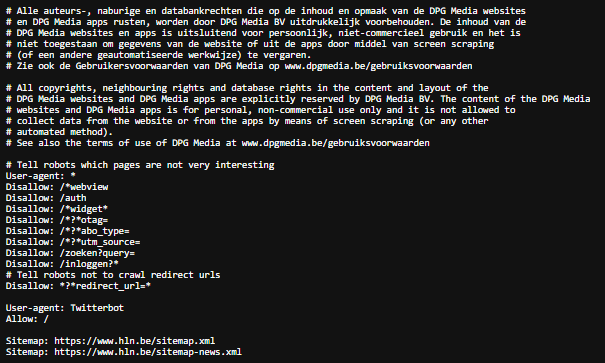
\includegraphics[width = 3in]{robotstxt_hln}
    \captionof{figure}{voorbeeld: www.hln.be/robots.txt}
    \label{fig:robotstxt}
\end{center}

\subsection{Wat is DALL-E (2)?}

\noindent
DALL-E is een AI software ontwikkeld door openAI dat beelden creëert uit tekstuele beschrijvingen, ook wel \emph{prompts} genoemd. Het gebruikt een versie met 12 miljard parameters van het GPT-3 Transformer-model om natuurlijke taalinvoer te interpreteren en overeenkomstige beelden te genereren. In april 2022 heeft OpenAI DALL-E 2 gelanceerd, ontwikkeld om meer realistische foto's met hogere resolutie te kunnen genereren. \\
 \autocite{DallEWikipediaNL}  \autocite{DallEWikipediaEN}\\

\noindent
DALL-E 2 is bovendien getrained met behulp van 650 milioen tekstinputs gescraped van het internet. \autocite{Borji2022} \\

\noindent
DALL-E 2 is niet open source maar kun je gebruiken aan de hand van de openAI API.  \\
\subsection{Wat is Stable Diffusion?}
\noindent
Stable Diffusion is een deep learning, tekst-naar-beeld model uitgebracht in 2022. In tegenstelling tot DALL-E (2) is Stable Diffusion getrained aan de hand van een diepe generatieve neurale netwerk.
\autocite{StableDifWikipediaEN}

Stable Diffusion is open source en kun je lokaal draaien op een computer met een GPU.



%---------- Methodologie ------------------------------------------------------
\section{Methodologie}%
\label{sec:methodologie}
\noindent
\textbf{Inleiding} \\
Het toegepaste onderzoek start op 2 maart 2023 en eindigt voor 28 mei 2023.

\noindent
\textbf{Fase 1: Realiseren van een scraper} \\
Om de data te bekomen van de verschillende soorten websites of social-media platformen zal er een web scraper worden gemaakt. Deze scraper zal ontwikkeld worden in python met behulp van een externe library \emph{BeautifulSoup}.

\noindent
\textbf{Fase 2: Data verwerken en analyseren} \\
Tijdens de tweede fase zullen we onderzoeken op welke manier we de bekomen data uit voorgaande fase kunnen analyseren en sorteren. \\ \\
\noindent
Het zal belangrijk zijn om rekening te houden met de volgende vragen: 
\begin{itemize}
    \item Wat zijn de te extraheren kernzaken?
    \item Wat is het sentiment van de dag? 
    \item Welke topic komt het vaakst voor?
    \item Op basis van welke gegevens kunnen we de artikels sorteren? 
\end{itemize}

\noindent
Nadat er een gepaste methode wordt gevonden om dit te realiseren, zal deze ook geïmplementeerd worden. Op deze manier kunnen we steeds het belangrijkste artikel van de dag eruit halen. \\

\noindent
\textbf{Fase 3: Kunstwerk genereren} \\
Nu dat we weten uit de vorige fase wat het hoogtepunt van de dag was. Kunnen we hierop een kunstwerk laten genereren. \\
Hiervoor zal er gebruik gemaakt worden van een of meerdere deep learning modellen DALL-E 2 en/of Stable Diffusion die de kerntekst van een artikel zal omvormen tot een foto. \\

\noindent
\textbf{Fase 4: Turing test} \\ 
Tijdens de laatste fase van dit onderzoek willen we bepalen of de AI-gegenereerde kunstwerken van DALL-E 2 en/of Stable Diffusion herkenbeer zijn uit het dagelijks nieuws. We zullen hiervoor een Turing test uitvoeren dit dit zal beoordelen.
%---------- Verwachte resultaten ----------------------------------------------
\section{Verwacht resultaten}%
\label{sec:verwachte_resultaten}
Het doel van het project is om een goed functionerende applicatie te ontwikkelen die dagelijks een kunstwerk kan genereren op basis van het hoogtepunt van de dag. Bijvoorbeeld, wanneer Marokko won van België tijdens de WK, kan het hoogtepunt in België \emph{'Riots in Brussels after soccer game, painting'} zijn. Op basis van deze tekstinput kunnen enkele voorbeelden gegenereerd worden met behulp van DALL-E 2. Deze voorbeelden worden weergegeven in de onderstaande afbeeldingen.


\noindent
\begin{tabular}{llll}
    \label{fig:examples}
    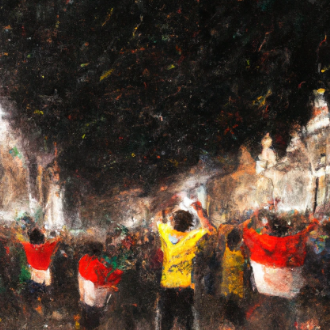
\includegraphics[width = 1.5in]{rellen_1.png} &
    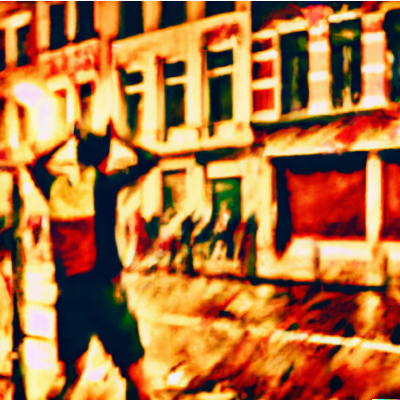
\includegraphics[width = 1.5in]{rellen_2.png} \\
    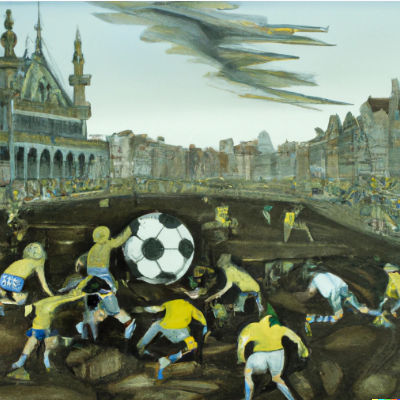
\includegraphics[width = 1.5in]{rellen_3.png} &
    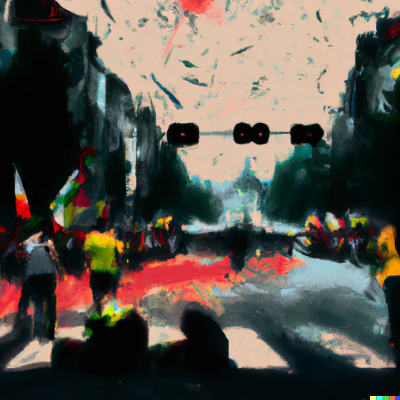
\includegraphics[width = 1.5in]{rellen_4.png}
\end{tabular} \\
\noindent
Daarnaast zal uit de turing test blijken of het kunstwerk enige boodschap overbrengt van het nieuws.
\noindent
Een voorbeeld van het resultaat van het project zou bijvoorbeeld kunnen zijn dat op een dag het hoogtepunt een artikel is over een nieuwe doorbraak in de gezondheidszorg. De applicatie zal dan op basis van de tekst van dat artikel een kunstwerk genereren dat hierbij past. In de verwachte resultaten zou dan bijvoorbeeld een afbeelding kunnen worden opgenomen van het gegenereerde kunstwerk op basis van enkele hoogtepunten van de dag. Als de gebruiker hier enige nieuws in kan herkennen en duidelijk kan verwoorden. Dan is dit een geslaagde test. 



%%---------- Andere bijlagen --------------------------------------------------
% TODO: Voeg hier eventuele andere bijlagen toe. Bv. als je deze BP voor de
% tweede keer indient, een overzicht van de verbeteringen t.o.v. het origineel.
%\input{...}

%%---------- Backmatter, referentielijst ---------------------------------------

\backmatter{}

\setlength\bibitemsep{2pt} %% Add Some space between the bibliograpy entries
\printbibliography[heading=bibintoc]

\end{document}
